%!TEX root = ../thesis.tex
%*******************************************************************************
%*********************************** Fifth Chapter *****************************
%*******************************************************************************

\chapter{Results and Discussions}
\graphicspath{{5_Results/Figs/}}

%This chapter summarise the results of the analysis in this project. 


%********************************** %First Section  **************************************
\section{ToT and Cluster Size Distributions} 
\label{section5.1}
Runs with varying pixel bias voltages and readout thresholds were analysed to obtain the distributions of time-over-threshold (ToT) and cluster size. This step is a quality assurance check, verifying that the observed trends with respect to changes in bias and threshold voltages are consistent with expectations.

Each ToT distribution was fitted with a Landau–Gaussian convolution to extract the peak value, representing the most probable charge deposition. For the cluster size distribution, the mean cluster size was calculated as a measure of the overall distribution, and charge sharing effect may be estimated. As shown in Fig. \ref{img:SingleRun}, the distribution was dominated by single-pixel clusters. While charge sharing was evident, the entries of larger clusters decreased rapidly with increasing size.

\begin{figure}[h!]
\centering
\begin{subfigure}[b]{0.49\linewidth}
  \centering
  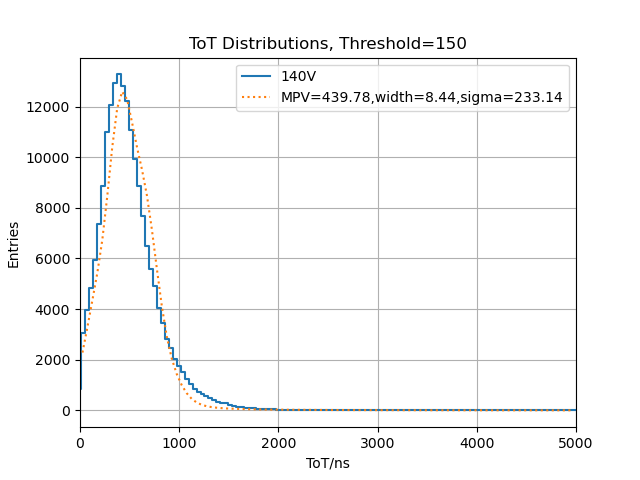
\includegraphics[width=1.0\linewidth]{TotDis}
  \caption{The distribution of ToT.}
\end{subfigure}
\begin{subfigure}[b]{0.49\linewidth}
  \centering
  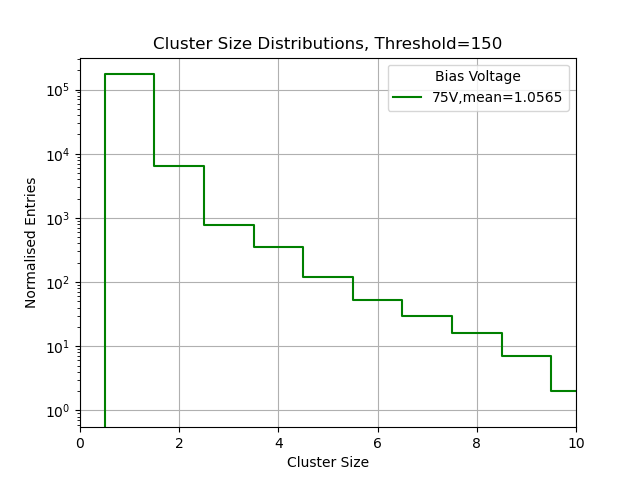
\includegraphics[width=1.0\linewidth]{ClusDis}
  \caption{The distribution of cluster sizes.}
\end{subfigure}
\caption{The distributions from a run with bias voltage 75V and threshold 150 DAC.}
\label{img:SingleRun}
\end{figure}

Next, the peak ToT values were compared cross different bias voltages and thresholds in Fig. \ref{img:TotVsThres}. In general, the peak value increases with higher bias voltage, due to increased charge production in a wider depletion zone, as expected. Conversely, the peak ToT decreases with higher threshold: for a given signal, a higher threshold reduces the time the signal remains above threshold. The outliers may result from unstable fits of the convoluted Landau-Gaussian function, which were not further refined due to time constraints.


\begin{figure}[h!] 
\centering    
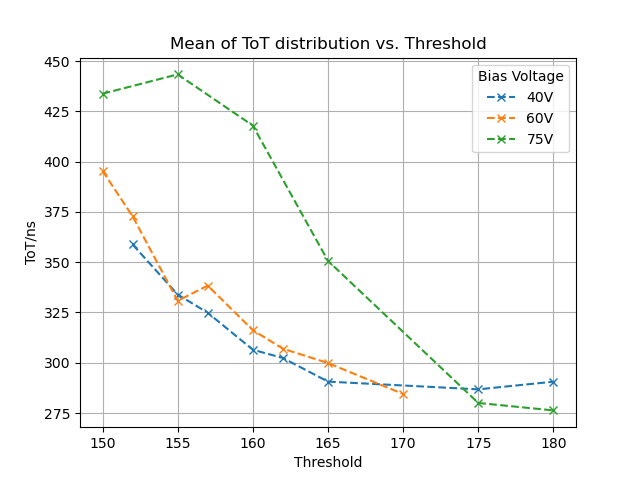
\includegraphics[width=0.7\linewidth]{TotVsThres}
\caption{A plot of the mean ToT value of the fitted Landau distribution versus the threshold.}
\label{img:TotVsThres}
\end{figure}


\begin{figure}[h!] 
\centering    
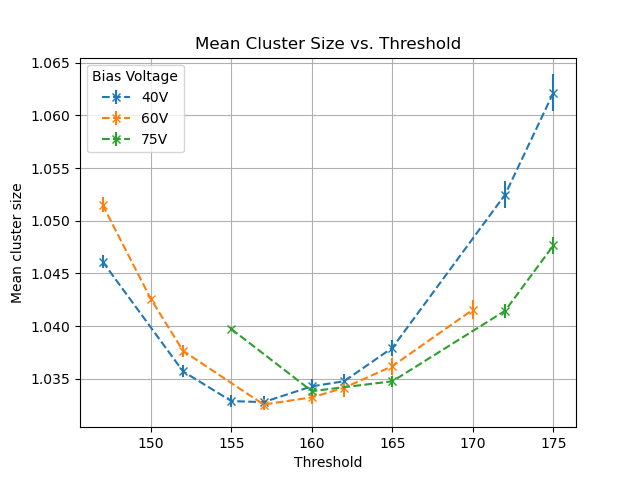
\includegraphics[width=0.7\linewidth]{ClusVsThres}
\caption{A plot of the mean cluster size versus the threshold.}
\label{img:ClusVsThres}
\end{figure}

A similar comparison was performed for the mean cluster size in Fig. \ref{img:ClusVsThres}. A minimum appears around a threshold of approximately 155–165 DAC, consistently observed across all bias voltages, with the position of the minimum shifting horizontally. A possible explanation is that, at these threshold values, noisy pixels near a real cluster fall below the threshold and are therefore not registered. When the threshold is further increased, single-pixel clusters begin to be suppressed, leaving only clusters with very large charge deposits and size. This leads to a rise in the mean beyond the minimum and a reduction to the number of events, as indicated by the larger error bars. This observation has also been reported in a separated experiment of TelePix2\cite{Emma}.

%On the other hand, the mean is generally expected to decrease with increasing bias voltages due to higher drift velocity. This trend is indeed observed for threshold $\geq$ 165 DAC. 

Overall, the performance of TelePix2 was stable and largely consistent with expectations, though improvements to the fittings are suggested.


%********************************** %Second Section  *************************************
\section{Efficiency} 
\label{section5.2}
To determine the optimal combination of bias voltage and threshold that gives the most reliable data for timing measurements, the efficiency defined in Eq. \ref{eq:Efficiency} was calculated.


\begin{figure}[h!] 
\centering    
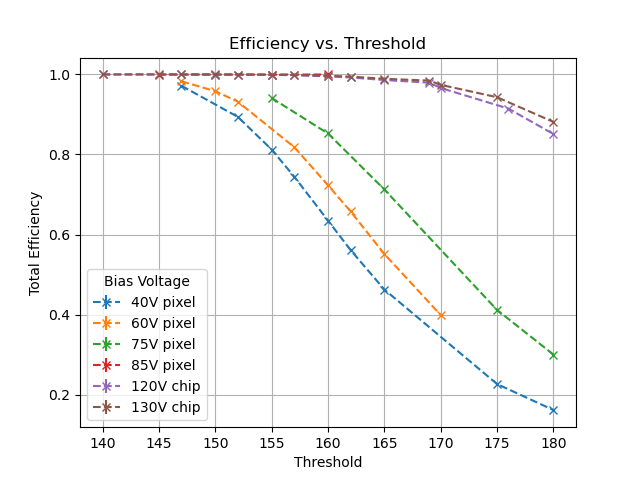
\includegraphics[width=0.7\linewidth]{EffVsThres}
\caption{The plot of efficiency versus threshold, at different bias voltages: 40-85 V pixel bias (on irradiated sensors), 120-130 V chip bias (on not-irradiated sensors). The difference between pixel and chip bias is given in Appendix \ref{appendix:bias}.}
\label{img:Efficiency}
\end{figure}

The sensor demonstrated good performance (efficiency$\geq$96\%) for threshold voltages below 160 DAC and bias voltages$\geq$85 V. Based on these observations, the run with a bias voltage 130 V, threshold 140 DAC was chosen to calculate the time resolution. 

Additionally, the results for pixel bias were obtained with sensors irradiated to a fluence of $1\times10^{14} n_{eq}$, demonstrating good radiation tolerance. It also suggests that a pixel bias above 85 V is required to ensure reliable operation, as the sensor accumulates radiation damage over its lifetime.


%********************************** % Third Section  *************************************
\section{Time-walk Correction}  
\label{section5.3}

As described in Sec. \ref{section:timewalk}, the time-walk effect requires correction in low ToT regions where it is significant. However, within the relevant range in the chosen run, the statistics was very limited - approximately 1\% of the entries fall within this region. This indicates that with an appropriate threshold, time-walk correction is not necessary for TelePix2 test beam.

\begin{figure}[h!] 
\centering    
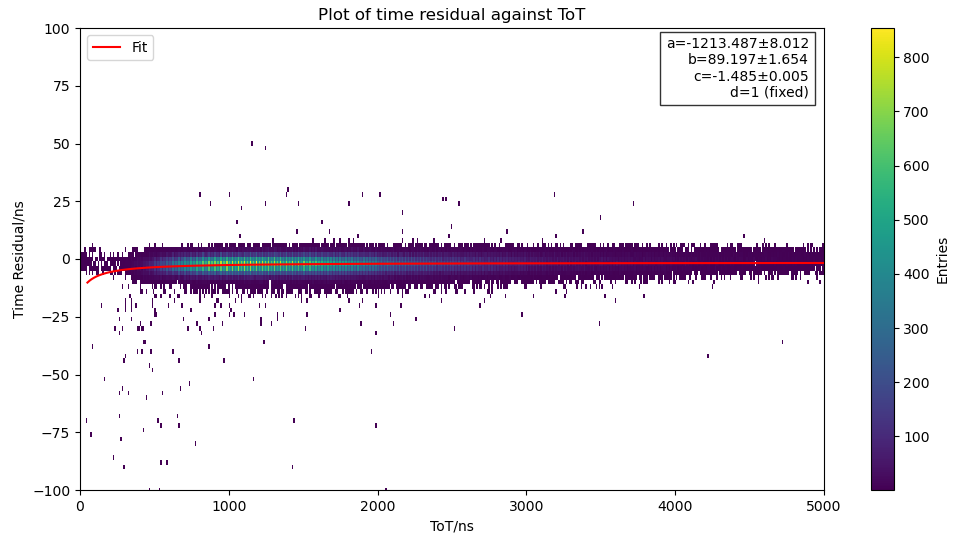
\includegraphics[width=0.9\linewidth]{TWalk}
\caption{The 2D histogram of time residual versus Time-over-Threshold(ToT).}
\label{img:Timewalk}
\end{figure}


\begin{figure}[h!] 
\centering
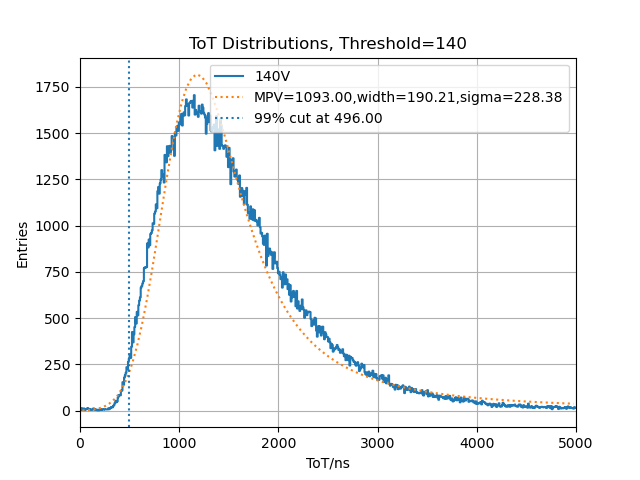
\includegraphics[width=0.65\linewidth]{TWalkInt}
\caption{The plot of efficiency versus threshold, at different values of bias voltage.}
\label{img:TimewalkIntegrate}
\end{figure}

It is worth noting that the time-walk effect becomes increasingly pronounced at higher thresholds. For a fixed bias voltage, the effect becomes noticeable from approximately 150 DAC onwards.



%********************************** % Fourth Section  *************************************
\section{Time Resolution}  
\label{section5.4}

A Gaussian curve was fitted to the time residual distribution for the chosen run. The time resolution was measured to be $2.656 \pm 0.003$ns, which satisfied the requirement of <3 ns.

\begin{figure}[h!] 
\centering    
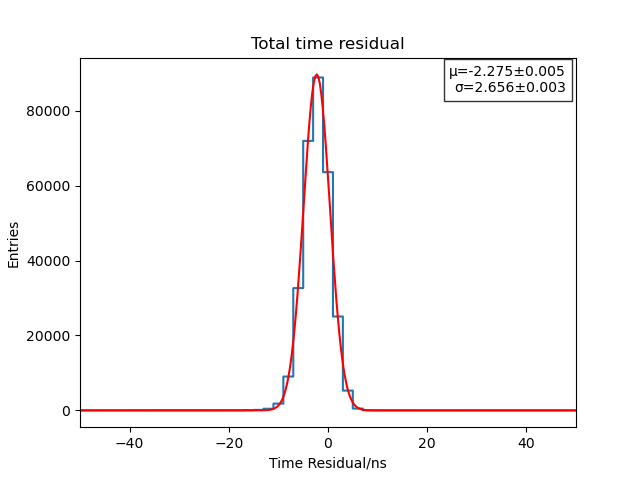
\includegraphics[width=0.8\linewidth]{TRes}
\caption{Time resolution of TelePix2, with chip bias voltage 130V, threshold 140 DAC.}
\label{img:TimeResolution}
\end{figure}


%********************************** % Fifth Section  *************************************
\section{In-pixel Spatial Correlation}  
\label{section5.5}

Finally, the entries of 1-pixel and 2-pixel clusters were plotted as a function of the in-pixel x position to investigate the charge-sharing effect. It is clear in Fig. \ref{img:InPixel} that the frequency of 1-pixel clusters decreases towards pixel edges, where charge-sharing is more likely to occur. However, the distribution of 2-pixel clusters has low statistics and does not exhibit a clear positional trend, suggesting the need for a longer data taking.

\begin{figure}[h!] 
\centering    
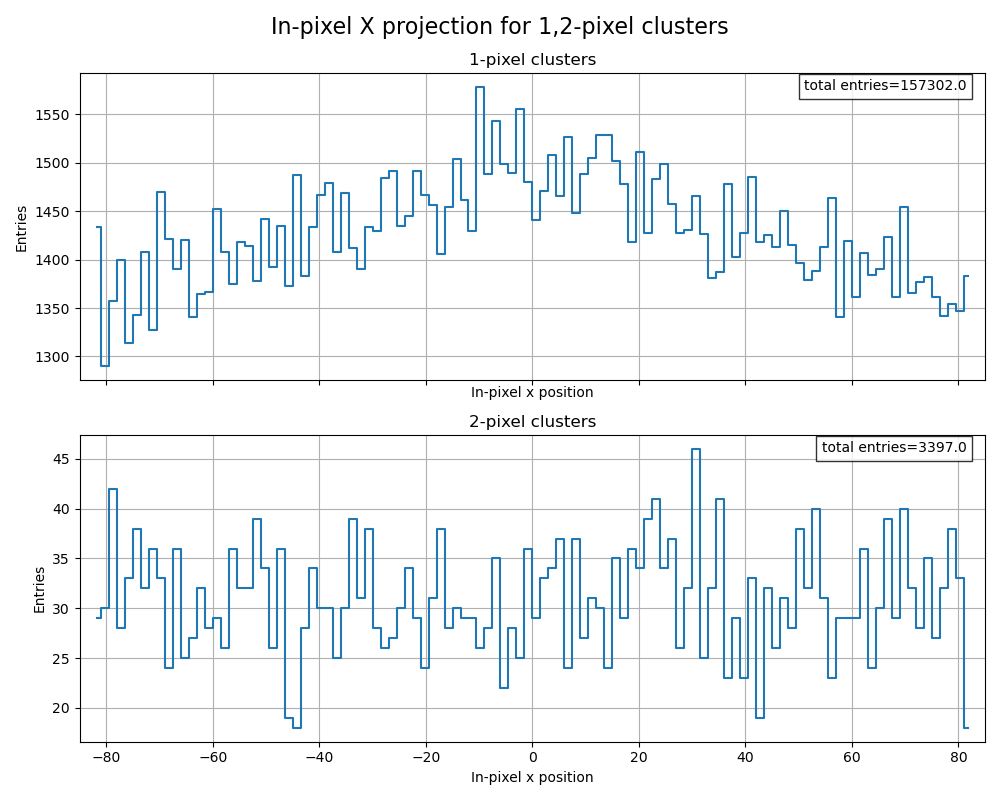
\includegraphics[width=0.9\linewidth]{InPixel}
\caption{A plot of the cluster entries versus their x-positions inside a pixel, for 1-pixel and 2-pixel clusters.}
\label{img:InPixel}
\end{figure}